\chapter{La Complicaci\'on: Restricci\'on de Estacionalidad en los Campos}

Todas las soluciones anteriores suponen que el agente al final de la cadena (el proveedor de materias primas) tiene inventario infinito. ¿Y si no fuera as\'i?

... que los campos tengan una restricci\'on temporal y solamente produzcan en los ciclos naturales de la cebada

Incluir aqu\'i la imagen de los ciclos naturales de la cebada en la figura \ref{fields}

\begin{figure}[h]
\caption{ }
\label{fields}
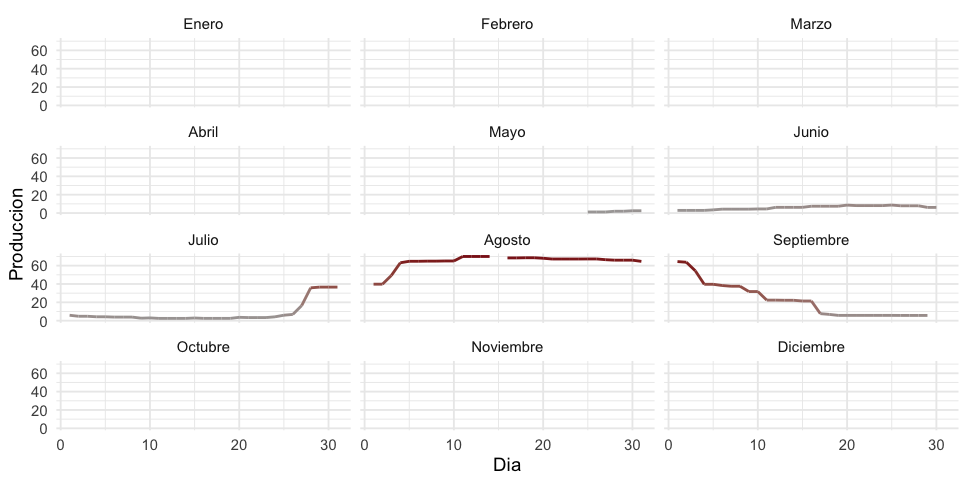
\includegraphics[width=13cm]{fields_monthly_supply_ggplot.png}
\centering
\end{figure}

En la figura \ref{analytic_3} podemos ver el comportamiento de la demanda (el cual fue descrito en cap\'itulos anteriores) en rosa y el de los campos, en verde. En este escenario se pueden observar varios efectos: 
\begin{itemize}
    \item Cada agente cuenta con inventario inicial, as\'i que tarda en comenzar a hacer pedidos al agente inmediatamente superior
    \item Cada agente deja de pedirle al agente inmediatamente superior cuando el segundo ya no tiene inventario. Esto es especialmente notorio para la f\'abrica: comienza a tener demanda positiva cuando ya hay producci\'on en los campos, cerca del d\'ia 150
    \item Si la oferta es m\'as baja que la demanda, los agentes piden todo lo que haya disponible, pues es preferible cubrir la demanda parcialmente que no cubrirla en lo absoluto
    \item Los agentes se preparan adecuadamente para el pico de septiembre, con un poco m\'as de anticipaci\'on a medida que se encuentran m\'as lejos del consumidor
\end{itemize}

\begin{figure}[h!]
\caption{Distribuci\'on de Cerveza}
\label{analytic_3}
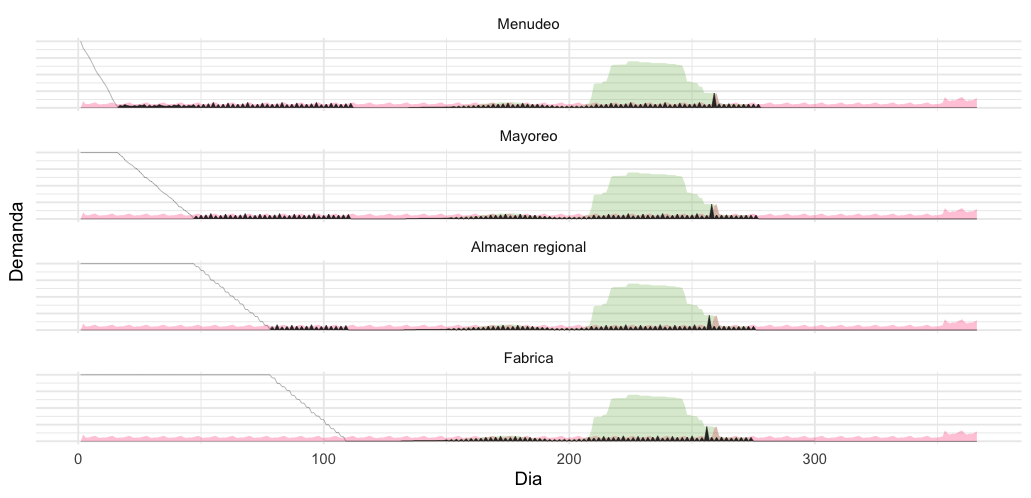
\includegraphics[width=16cm]{tesis_tex/figs/analytic_with_fields_restriction.png}
\centering
\end{figure}

Sin embargo, los agentes no se prepararon adecuadamente para cubrir la demanda posterior al tiempo en que los campos tuvieron producci\'on positiva. Esto sucede porque, en este modelo, los agentes ven solamente un periodo hacia el futuro, as\'i que solo se preparan para ese d\'ia. Esta complicaci\'on vuelve imperante que todos los agentes usen sus almacenes para poder afrontar la demanda, incluso cuando no hay producci\'on.

En este trabajo presentaremos un modelo con esta restricci\'on, y lo resolveremos tanto con \textit{policy iteration} como con \textit{Q-learning}.
